% scan design
\begin{frame}{Signal Model}
	\alt<1>{%
		After reconstruction, 
			single voxel $y_d$ in $d$th image modeled as \\
		\begin{align}
			y_d = s_d\paren{\bmx; \bmnu, \bmp_d} + \epsilon_d
		\end{align}
	}{%
		A \emph{scan profile} is a set of $D$ scans
			that produces at each voxel \\
			a measurement vector $\bmy := \brac{y_1,\dots,y_D}\tpose$ 
			modeled as
			\begin{align}
				\bmy = \bms\paren{\bmx; \bmnu, \bmP} + \bmeps
			\end{align}
	}
	\begin{itemize}
		\item<1>{\makebox[3.5cm][l]{$\bmx \in \reals{L}$} unknown parameters}
		\item<1>{\makebox[3.5cm][l]{$\bmnu \in \reals{K}$} ``known'' parameters}
		\alt<1>{%
			\item<1>{\makebox[3.5cm][l]{$\bmp_d \in \reals{A}$} acquisition parameters}
			\item<1>{\makebox[3.5cm][l]{$s_d : \reals{L+K+A} \mapsto \complex$} 
				$d$th signal model
			}
			\item<1>{\makebox[3.5cm][l]{$\epsilon_d \in \complex$} 
				noise $\sim \cgauss{0}{\sigma_d^2}$
			}
		}{%
			\item<2>{\makebox[3.5cm][l]{$\bmP := \brac{\bmp_1,\dots,\bmp_D}$} 
				acquisition parameter matrix
			}
			\item<2>{\makebox[3.5cm][l]{$\bms : \reals{L+K+AD} \mapsto \complexes{D}$}
				vector signal model
			}
			\item<2>{\makebox[3.5cm][l]{$\bmeps \sim \cgauss{\zeros{D}}{\bmSig}$}
				noise, with $\bmSig := \diag{\sigma_1^2,\dots,\sigma_D^2}$ 
			}
		}
	\end{itemize}
	\uncover<3->{%
		\textbf{Task}: design $\bmP$ to enable precise unbiased estimation of $\bmx$
	}
\end{frame}

\begin{frame}{Towards an Objective Function}
	\uncover<1>{%
  	When $\bms$ is analytic in $\bmx$ (as is typical), \\
  	\textbf{Fisher information} characterizes unbiased estimator precision:
  	\begin{align}
  		\bmF\paren{\bmx; \bmnu, \bmP} := 
  			\paren{\grada{\bmx} \bms\paren{\bmx; \bmnu, \bmP}}\ctpose
  			\bmSig^{-1} \grada{\bmx} \bms\paren{\bmx; \bmnu, \bmP}.
  	\end{align}
  }%
  \uncover<2-3>{%
  	When $\bmF$ is invertible, \Cramer-Rao Bound (CRB) \hfill \citec{cramer:46} \\
  	ensures covariance of unbiased estimates $\est{\bmx}$ of $\bmx$ satisfy
  	\begin{align}
  		\cov{\est{\bmx}; \bmnu, \bmP} \succeq \bmF^{-1}\paren{\bmx; \bmnu, \bmP}.
  	\end{align}
	}%
	\uncover<2>{%
  	Maximum-likelihood (ML) estimates achieve CRB asymptotically \\
  	or (equivalently for Gaussian data) at sufficiently high SNR. \\
	}%
	\uncover<3>{%
		\textbf{Idea}: choose $\bmP$ such that imprecision matrix $\bmF^{-1}$ ``small''
	}
\end{frame}

\begin{frame}{Scan Design}
	\uncover<1-4>{%
		\textbf{Idea}: choose $\bmP$ to minimize the objective 
		\begin{align}
			\costa{\bmx; \bmnu, \bmP} =
        \trace{\bmW \bmF^{-1}\paren{\bmx; \bmnu, \bmP} \bmW\tpose},
		\end{align}
	where $\bmW \in \reals{L\times L}$ is a pre-selected diagonal matrix of weights.
	}%
	\uncover<2>{%
		\textbf{Challenge}: $\bmx,\bmnu$ vary spatially \\
	}
	\uncover<3->{%
  	\textbf{Two problems considered}: 
  	\begin{itemize}
  		\item<3-5>{%
  			min-max scan design \hfill \citec{nataraj:17:oms}
  			\begin{align}
  				\breve{\bmP} &\in \set{
  					\argmin{\bmP \in \setP}
  					\max_{\substack{\bmx \in \setXt \\ \bmnu \in \setNt}}
  					\costa{\bmx; \bmnu, \bmP}
  				}
  			\end{align}
  		}%
			\only<3>{%
				where $\setXt \subseteq \reals{L}$ and $\setNt \subseteq \reals{K}$ 
				are ``tight'' ranges of interest \\
				and $\setP$ is defined by acquisition/timing constraints \\
			}%
  		\item<4>{%
  			Bayesian scan design
  			\begin{align}
  				\breve{\bmP} &\in \set{
  					\argmin{\bmP \in \setP}
  					\expect{\bmx,\bmnu}{\costa{\bmx; \bmnu, \bmP}}
  				}
  			\end{align}
  		}%
  	\end{itemize}
	}
\end{frame}

\begin{frame}{Detailed Example Study}
	\uncover<1->{%
		\textbf{Task}: design fast acquisition for precise estimation 
			of relaxation parameters $\To,\Tt$ in white/gray matter (WM/GM) of brain
	}
	\begin{itemize}
		\item<2>{Consider scan profiles consisting of two fast pulse sequences}
		\begin{itemize}
			\item{Spoiled Gradient-Recalled Echo (SPGR) \hfill \citec{zur:91:sot}}
			\item{Dual-Echo Steady-State (DESS) \hfill \citec{redpath:88:fan}}
		\end{itemize}
		\item<3>{For each scan profile feasible under total time constraint:}
		\begin{enumerate}
			\item{Let $\bms$ model corresponding single-component signal}
			\begin{itemize}
				\item{$\bmx \gets \brac{\mzero, \To, \Tt}\tpose$}, 
					where $\mzero$ is a scale factor
				\item{$\bmnu \gets$ flip angle variation}
				\item{$\bmP \gets$ nominal flip angles, repetition times}
			\end{itemize}
			\item{Optimize $\bmP$ subject to flip angle, sequence timing constraints}
			\begin{itemize}
				\item{$\bmW \gets \diag{0, 0.1, 1}$ emphasizes $\To,\Tt$ est roughly equally}
				\item{$\setXt$ chosen to focus on WM/GM at 3T field strength}
				\item{$\setNt$ chosen to allow 10\% flip angle variation}
			\end{itemize}
		\end{enumerate}
	\end{itemize}
\end{frame}

\begin{frame}{Scan Profile Comparison}
	\uncover<1>{%
  	\begin{table}
      \centering
      {\tabulinesep = 0.5mm
      \begin{tabu} {r | c c c}
         \hline \hline
         (\#SPGR, \#DESS) Profiles & $(2,1)$ & $(1,1)$ & $(0,2)$ \\
         \hline
         SPGR nom. flip (deg) & (15, 5) & 15 & -- \\
         DESS nom. flip (deg) & 30 & 10 & (35, 10) \\
         SPGR rep. times (ms) & (12.2, 12.2) & 13.9 & -- \\
         DESS rep. times (ms) & 17.5 & 28.0 & (24.4, 17.5) \\
         \hline
         \textbf{optimal max cost} & 4.0 & 4.9 & \textbf{3.5} \\
         \hline \hline
  		\end{tabu}}
			\label{table:profile}
  	\end{table}
	}%
	\uncover<2>{%
		\textbf{Main finding}: 
			2 DESS sequences can yield $\To,\Tt$ WM/GM estimates 
			that are at least as precise as $\To,\Tt$ estimates 
			from SPGR/DESS scan profiles, 
			under this competitive time constraint.
	}%
\end{frame}

\begin{comment}
\begin{frame}{Numerical Simulation}
	\uncover<+->{%
		\begin{itemize}
			\item{Simulated many WM-like, GM-like voxel realizations}
			\item{Studied sample statistics of $\To,\Tt$ ML estimates $\ToML,\TtML$}
		\end{itemize}
	}
	\uncover<+->{%
  	\begin{table} [!tb]
      \centering
      {\tabulinesep = 0.2mm
      \begin{tabu} {c | r r r | r}
          \hline \hline
          Profile     & $(2,1)$           & $(1,1)$           & $(0,2)$           & Truth \\
          \hline
          WM $\ToML$  & $830 \pm 17$      & $830 \pm 15$      & $830 \pm 14$      & $832$ \\
          GM $\ToML$  & $1330 \pm 30.$    & $1330 \pm 24$     & $1330 \pm 24$     & $1331$ \\
          \hline
          WM $\TtML$  & $80. \pm 1.0$     & $80. \pm 2.1$     & $79.6 \pm 0.94$   & $79.6$ \\
          GM $\TtML$  & $110. \pm 1.4$    & $110. \pm 3.0$    & $110. \pm 1.6$    & $110$ \\
          \hline \hline
      \end{tabu}}
      \caption{$\ToML,\TtML$ sample means $\pm$ sample standard deviations}
      \label{table:numerical}
  	\end{table}
	}
\end{frame}
\end{comment}

\begin{frame}{Experimental Setup}
	\uncover<1>{%
		Candidate $(2,1)$, $(1,1)$, $(0,2)$ SPGR/DESS scan profiles
		\begin{itemize}
			\item{Prescribed optimized nominal flip angles, repetition times}
			\item{Used $256 \times 256 \times 8$ 3D matrix 
				over $24 \times 24 \times 4$cm FOV}
			\item{Required \textbf{1m37s} scan time for each profile}
		\end{itemize}
	}
	\uncover<2>{%
		Reference scan profile
		\begin{itemize}
			\item{Four inversion recovery (IR) scans for $\To$ estimation}
			\item{Four spin-echo (SE) scans for $\Tt$ estimation}
			\item{$256 \times 256$ matrix over $24 \times 24 \times 0.5$cm FOV}
			\item{Required \textbf{40m58s} scan time total}
		\end{itemize}
	}
	\uncover<3>{%
		Bloch-Siegert (BS) acquisition for separate flip angle calibration
		\begin{itemize}
			\item{Acquired 2 BS-shifted 3D SPGR scans in 1m40s total}
			\item{Used for $\To,\Tt$ est from both candidate and reference profiles}
		\end{itemize}
	}
\end{frame}

\begin{frame}{Phantom Accuracy Results}
	\begin{figure}
		\centering
		\subfloat [$\ToML$ Estimates] {
        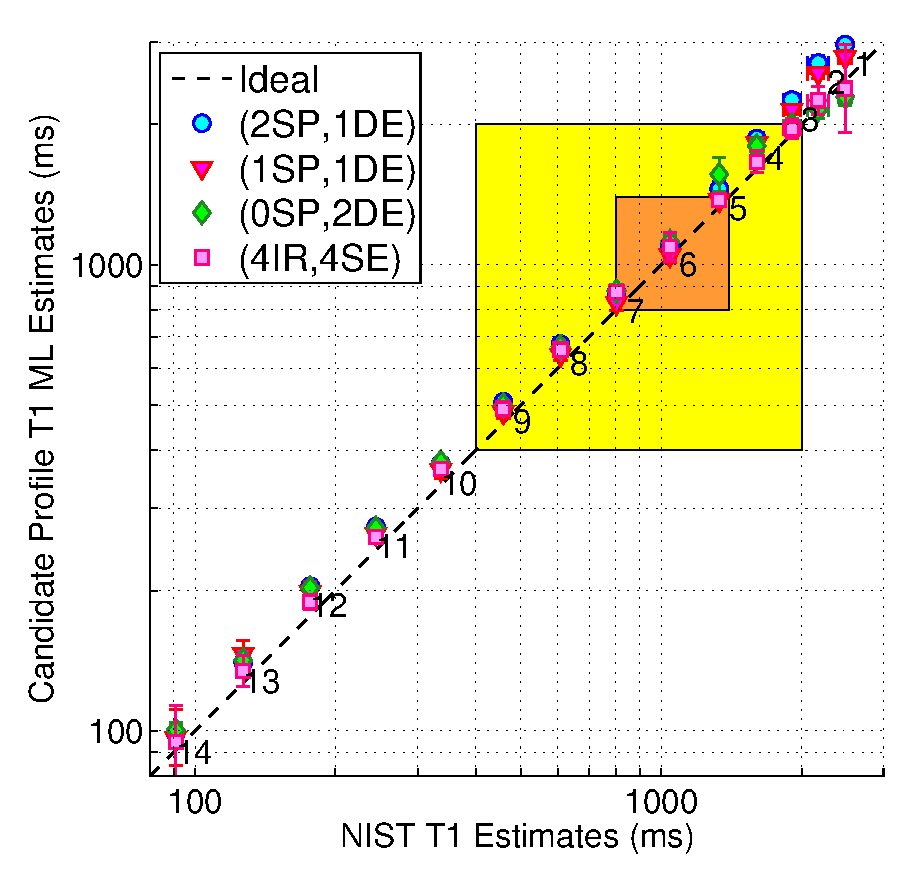
\includegraphics [width = 0.45\textwidth] 
        	{c,scn-dsgn/2016-06-20,hpd,t1-ml-compare.eps}
        \label{fig:scn-dsgn,hpd,t1}
    }
    \hspace{0.3cm}
    \subfloat [$\TtML$ Estimates] {
        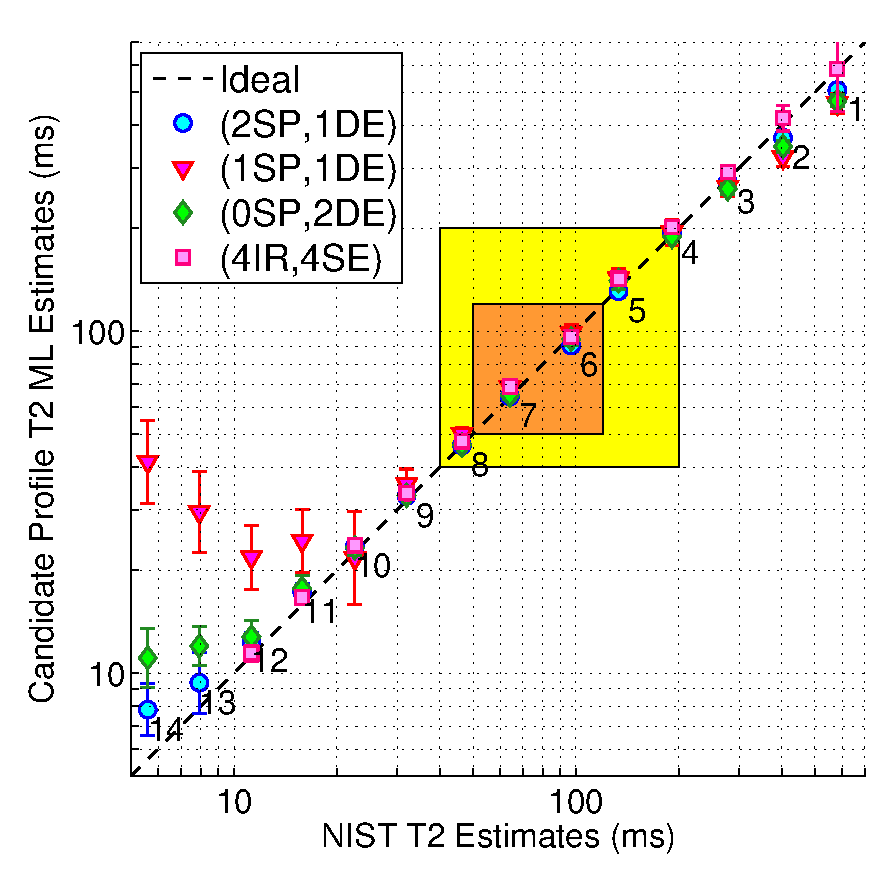
\includegraphics [width = 0.45\textwidth] 
        	{c,scn-dsgn/2016-06-20,hpd,t2-ml-compare.eps}
        \label{fig:scn-dsgn,hpd,t2}
    }
    \label{fig:scn-dsgn,hpd}
 	\end{figure}
	Compared against NIST NMR measurements \hfill \citec{keenan:16:msm}
\end{frame}

\begin{frame}{Phantom Precision Results}
	\only<1>{%
  	\begin{itemize}
  		\item{Repeated each profile 10 times}
  		\item{Estimated $\To,\Tt$ std dev of typical voxel across repetitions}
  	\end{itemize}
	}%
	\uncover<2>{%
  	\begin{table}
      \centering
      \begin{tabu} {c | r r r}
      	\hline \hline
        						    & (2, 1)         		& (1, 1)         		& (0, 2) \\
        \hline
        V5 $\sigToML$   & $50 \pm 12$       & $40 \pm 10.$    	& $39 \pm 9.4$ \\
        V6 $\sigToML$   & $70 \pm 18$       & $60 \pm 15$       & $60 \pm 16$ \\
        V7 $\sigToML$   & $60 \pm 13$       & $50 \pm 13$       & $50 \pm 13$ \\
        \hline 
        V5 $\sigTtML$   & $2.6 \pm 0.63$    & $6 \pm 1.4$       & $3.5 \pm 0.84$ \\
        V6 $\sigTtML$   & $1.9 \pm 0.46$    & $5 \pm 1.1$       & $2.3 \pm 0.54$ \\
        V7 $\sigTtML$   & $1.4 \pm 0.34$    & $3.4 \pm 0.80$    & $1.5 \pm 0.35$ \\
        \hline 
        $\sqrt{\textrm{opt max cost}}$ estimate
        								& $8.9 \pm 1.8$ 		& $11 \pm 2.6$ 			& $\mathbf{8.3 \pm 2.1}$ \\
        \hline \hline
      \end{tabu}
      \caption{
          Pooled sample standard deviations
          $\pm$ pooled standard errors of sample standard deviations (ms),
          from optimized SPGR/DESS profiles.
      }
      \label{table:hpd,sample-std-dev}
  	\end{table}
	}%
	\uncover<3>{%
		Similar trends across profiles of empirical vs. theoretical std dev!
	}
\end{frame}

\begin{frame}{Summary}
	\only<3>{%
		\vspace{-1cm}
  	\begin{figure}
  		\centering
  		\subfloat{
  			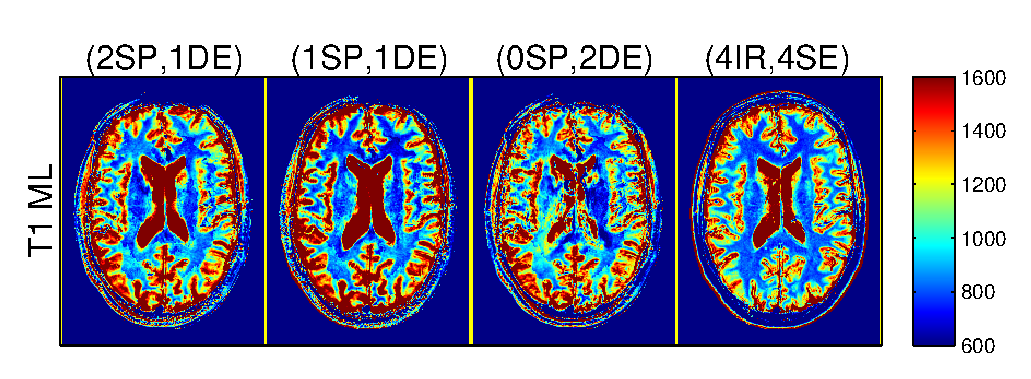
\includegraphics [width=\textwidth, trim=0 0 0 10, clip] 
  				{c,scn-dsgn/2016-05-31,brain,t1-ml,jet.eps}
  			\label{fig:scn-dsgn,brain,t1}
  		}
  		\vspace{0cm}
  		\subfloat{
  			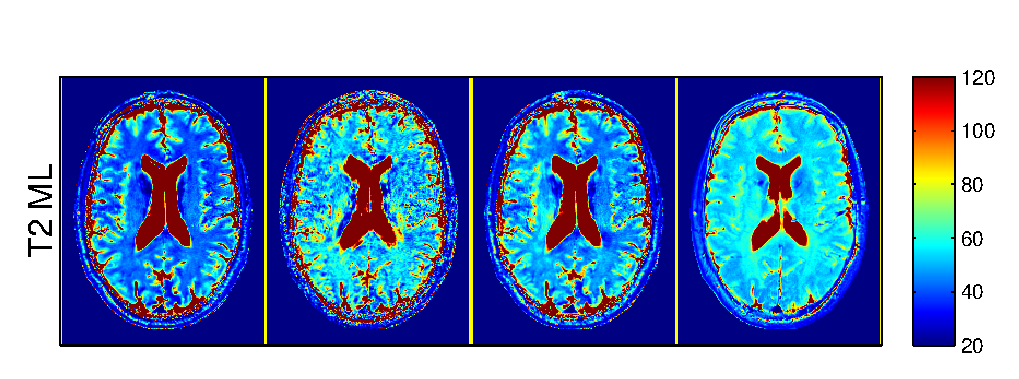
\includegraphics [width=\textwidth-1mm, trim=0 0 0 25, clip]
  				{c,scn-dsgn/2016-05-31,brain,t2-ml,jet.eps}
  			\label{fig:scn-dsgn,brain,t2}
  		}
  		\caption{
  			Colorbar ranges in ms.
  		}
  		\label{fig:scn-dsgn,brain}
  	\end{figure}
	}
	\only<1-2,4-5>{%
  	\uncover<1->{%
  		\textbf{Contributions}
  			\begin{itemize}
  				\item<1->{MR scan design method for precise parameter estimation}
  				\item<1->{Fast SPGR/DESS scan profile for $\To,\Tt$ estimation in brain}
  				\begin{itemize}
  					\item<2->{%
  						Phantom (and omitted simulation) results validate method \\
  						as a predictor of unbiased estimation precision.
  					}
  					\item<4->{
  						\emph{In vivo} results reveal discrepancies 
  						(especially in $\Tt$ estimates),
  						suggesting $\To,\Tt$ estimates sensitive to model mismatch.
  					}
  				\end{itemize}
  			\end{itemize}
  	}
  	\uncover<5>{%
  		\textbf{How to address \invivo model mismatch?}
  		\begin{itemize}	
  			\item{More accurate \invivo signal models}
  			\item{More scalable parameter estimation}
  		\end{itemize}
  	}
	}
\end{frame}
